\usepackage{textcomp}
\decimalpoint
%------------Diseño de página --------------------------------
\usepackage[centering, letterpaper,margin=2cm,top=1cm, headsep=24pt, headheight=2.5cm,includehead, includefoot]{geometry}

%------------Colores----------------------

\definecolor{principal}{RGB}{0, 157, 197}
\definecolor{secundario}{RGB}{43, 82, 96}
\definecolor{terciario}{RGB}{43,82,96}

%--------------Hipervinculos en color, ligas-azul, archivos-magenta, url-azul----------------
\hypersetup{
    colorlinks=true,
    linkcolor=secundario,
    filecolor=magenta,      
    urlcolor=blue}

%-------------Encabezado---------------------
\pagestyle{fancy}
\fancyhf{}

\chead{\begin{tabular}{m{14.2cm}m{2.5cm}}
\rowcolor{principal}
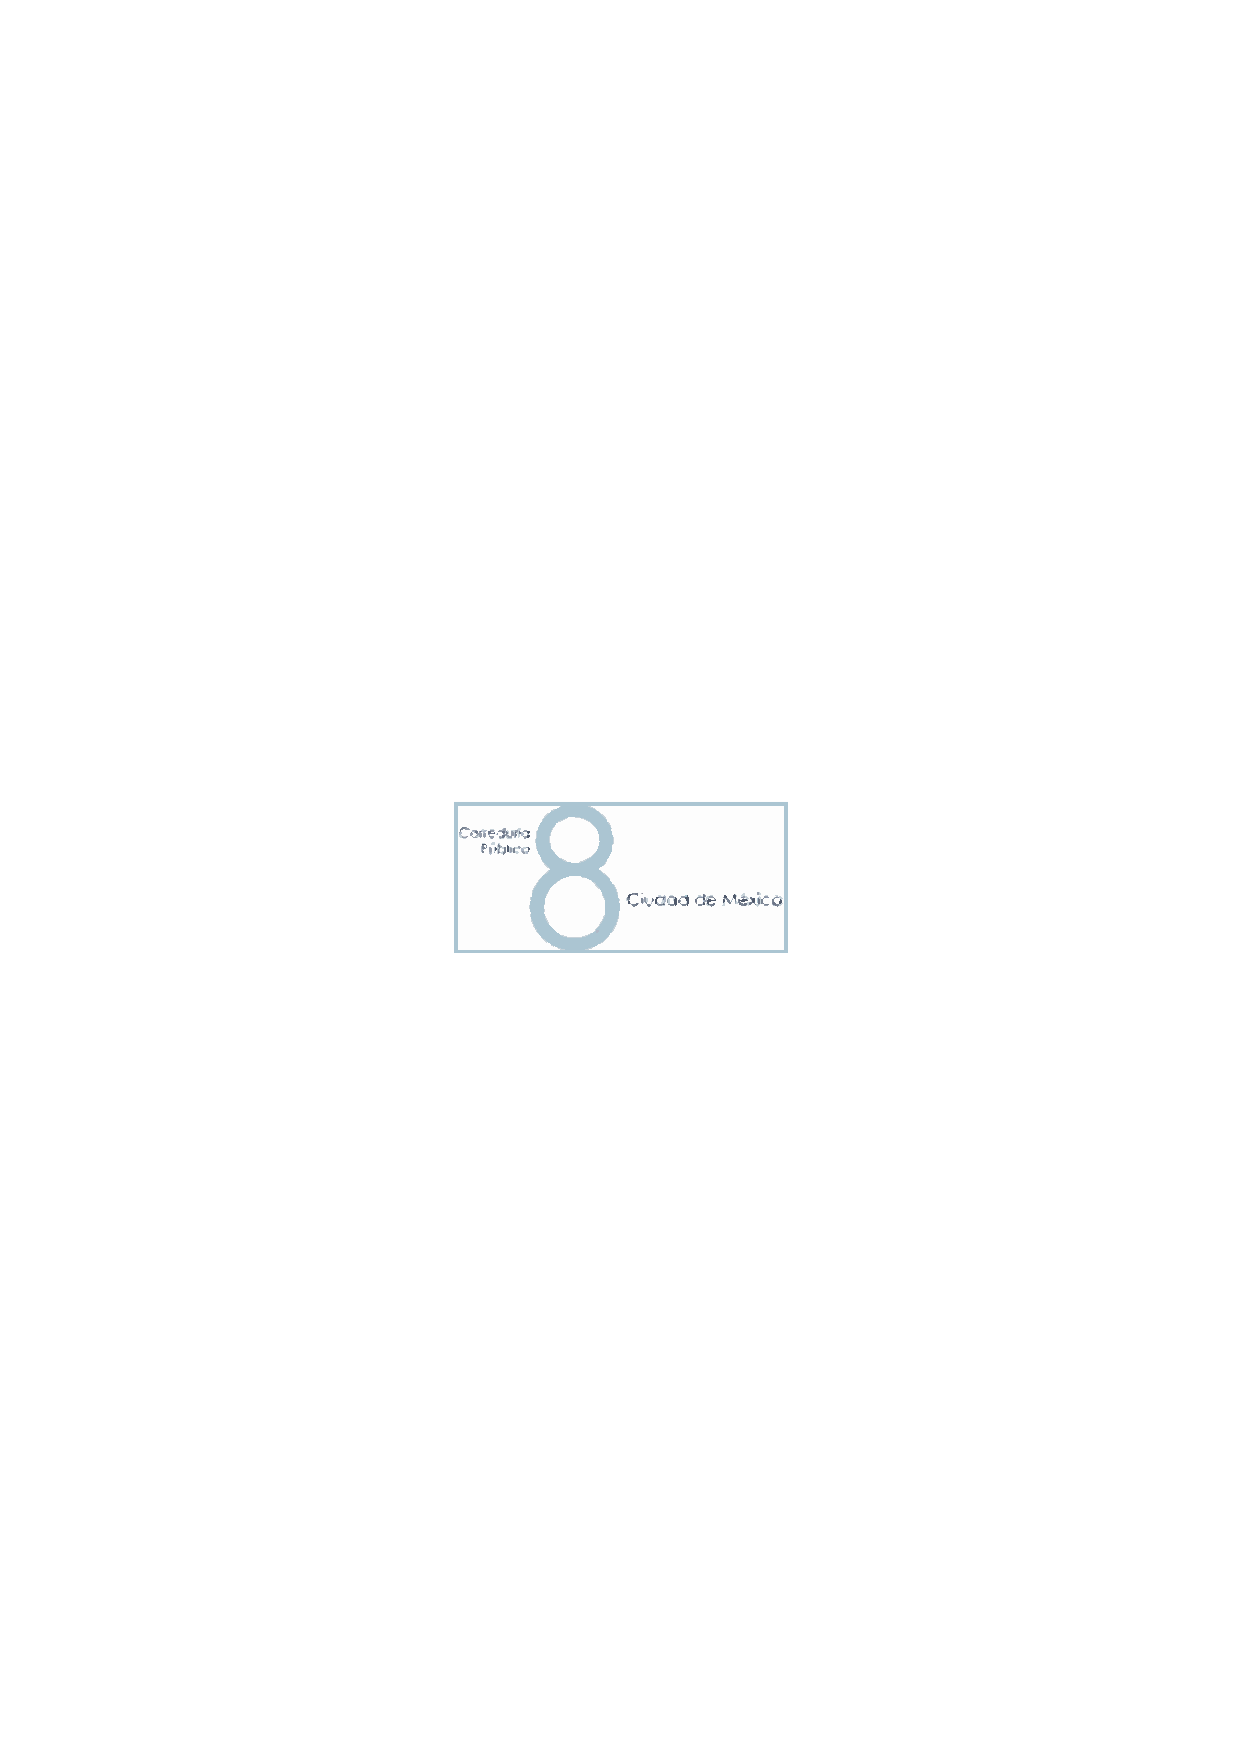
\includegraphics[width=4.5cm]{\rutaImagenes/logo_cp_8(2).pdf} &\\
\end{tabular}
}

%--------------Pie de página------------------
\cfoot{\textbf{\textcolor{principal}{\footnotesize{Corredur\'ia P\'ublica 8 Ciudad de M\'exico}}}\\ \scriptsize{\textit{Montes Urales 755 Piso 5, Col. Lomas de Chapultepec, Miguel Hidalgo,\\ CDMX, C.P. 11000. Tel. (55)41616060}}}
\rfoot{\footnotesize{\thepage\hspace{3pt}de \pageref{lastpage}}}
\lfoot{
\begin{tabular}{b{2cm}}

\includegraphics[width=1.5cm]{\rutaImagenes/qr}
\end{tabular}}

%------------Títulos de seccion y subseccion--------------



\renewcommand \thechapter {\Roman{chapter}}
\renewcommand \thesection {\Alph{section}}
\renewcommand \thesubsection {\thesection.\arabic{subsection}}
\renewcommand \thesubsubsection {\thesection.\arabic{subsection}.\arabic{subsubsection}}

\titleformat{\section}[hang]{\color{gray}\huge\bfseries}{\thesection.}{1em}{} 

\chapterfont{\color{principal}}
\sectionfont{\color{principal}}
\subsectionfont{\color{secundario}}
\subsubsectionfont{\color{terciario}}

\titleformat{\chapter}[display]{\normalfont\Large\filcenter\sffamily}
{\titlerule[1pt]%
\vspace{1pt}%
\titlerule
\vspace{1pc}%
\LARGE\MakeUppercase{\chaptertitlename} \thechapter}
{1pc}
{\titlerule
\vspace{1pc}%
\Huge}
\titlespacing{\chapter}{0pt}{*-8}{*1.5}

%------------------Profundidad del índice---------------------------

\setcounter{tocdepth}{3}
\setcounter{secnumdepth}{3}


%------------------Marca de agua---------------

\backgroundsetup{angle=0, contents={
\includegraphics[width=4cm]{\rutaImagenes/logo_cp_8}},opacity=.2, scale=2}
